\section{System Perspective}

%A description and illustration of the:

%  - Design and architecture of your _ITU-MiniTwit_ systems
%  - All dependencies of your _ITU-MiniTwit_ systems on all levels of abstraction and development stages.
%    - That is, list and briefly describe all technologies and tools you applied and depend on.
%  - Important interactions of subsystems
%  - Describe the current state of your systems, for example using results of static analysis and quality assessments.
%  - Finally, describe briefly, if the license that you have chosen for your project is actually compatible with the licenses of all your direct dependencies.

%Double check that for all the weekly tasks (those listed in the schedule) you include the corresponding information.

\subsection{Design and architecture}

The technologies we selected to recreate the legacy flask application ITU-MiniTwit, were C\# with the ASP.NET Core framework for the server and Postgresql as the database. The decision of using ASP.NET Core was made based on that the team had prior experience using it, which enabled us to quickly implement the features from the Flask application. Another reason for our selection is that with the performance enchancements of .NET 7, this is a very well performing framework\footnote{14th in this benchmark: 
\url{https://www.techempower.com/benchmarks/#section=data-r21}}. This can also be seen in our groups solution being one of the top performing in this chart: \url{http://104.248.134.203/chart.svg}.

We used Razor pages to render the web pages on the server side. We also considered creating a single page application as a frontend, such as with Blazor or React, as this would be the more modern approach. However we stuck to using Razor pages as we wanted to replicate the original Flask application as much as possible.

Figure \ref{fig:architecture} shows the architecture of the final version of the system that was deployed, using three droplets (virtual machine) on DigitalOcean. Docker containers are within a docker swarm and communicate via the internal overlay network. There are three replicas of the MiniTwit server in the swarm, one on each droplet, to ensure availability. The two worker nodes only contain an instance of the MiniTwit server, the manager contains the services for load balancing, logging and monitoring. We decided to keep all these services on the same node so they are accessible on the same IP address. Nginx is used for load balancing between the MiniTwit instances. The database was hosted as a DigitalOcean managed database so that it was guaranteed to be reliable. Initially, we managed the postgres database ourselves, however one day it suddenly crashed causing approximately 12 hours of downtime. To avoid worrying about this we decided to switch to a managed database in our deployment. Running our \textit{infrastructure.sh} script, which deploys the entire system and provisions the infrastructure on DigitalOcean, will make the database as a container in the swarm though.

\begin{figure}[H]
    \centering
    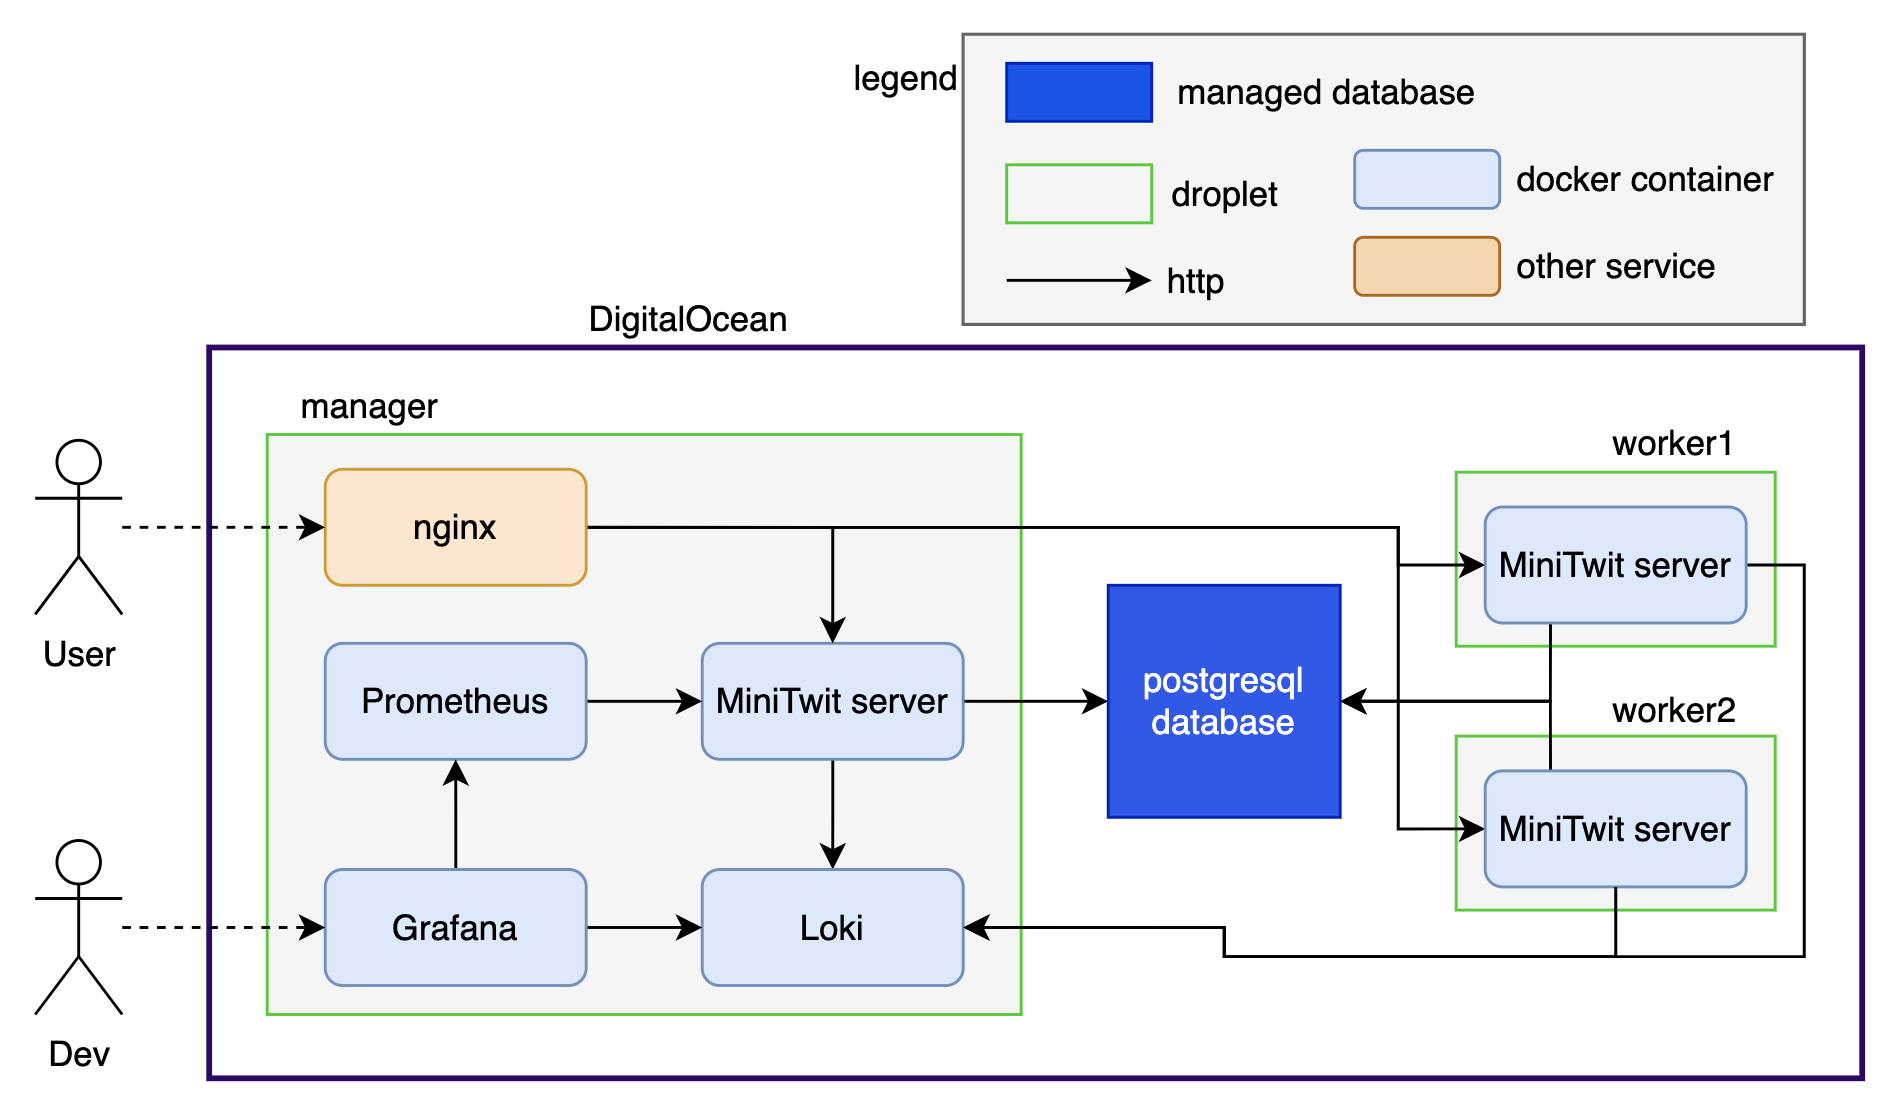
\includegraphics[width=\textwidth]{images/architecture.png}
    \caption{Architecture of the final system.}
    \label{fig:architecture}
\end{figure}

\subsection{Technologies and Dependencies}

The technologies we have decided on for the system to rely on are listed below. All versions used were the most recent stable releases as of start-2023:

\begin{itemize}
    \item \textbf{ASP.NET Core}, for the web application.
    \item \textbf{PostgreSQL}, for data storage.
    \item \textbf{nginx}, for reverse proxy and load balancing.
    \item \textbf{Grafana}, for view metrics and logs.
    \item \textbf{Loki}, for storing logs.
    \item \textbf{Prometheus}, for storing metrics.
    \item \textbf{Docker}, for containerization.
    \item \textbf{Docker Hub}, for container image registry.
    \item \textbf{Ubuntu}, for the server OS.
    \item \textbf{Python}, for the tests.
    \item \textbf{Nuget}, for package management.
    \item \textbf{Github Actions}, for CI/CD.
    \item \textbf{DigitalOcean}, for infrastructure.
    \item \textbf{SonarCloud}, for static analysis.
\end{itemize}

\noindent The libraries which the ASP.NET Core MiniTwit application depends on are:

\begin{outline}
    \1 \textbf{Entity Framework Core}, library for database abstraction layer.
    \1 \textbf{Npgsql}, library for connecting to postgres from .NET.
    \1 \textbf{Serilog}, library for logging.
    \1 \textbf{Serilog.Sinks.Grafana.Loki}, library for shipping logs to Loki.
    \1 \textbf{Prometheus-net}, library to instrument .NET code with Prometheus metrics.
    \1 \textbf{SignalR}, library for realtime communication between client and server.
\end{outline}

\subsection{Important interactions of subsystems}

Prometheus only read from the one of the MiniTwit server instances. Since the load is balanced this means that only 1/3 of the traffic is monitored by metrics. This is not optimal, since it does not give all of the information, however it does present a sort of snippet of the systems' monitoring.

\todo[inline]{Er der mere til interactions?}

\subsection{Current state of systems}
\todo[inline]{Indrag sonarcloud, Indrag screenshots fra grafana?}

Due to our project utilizing infrastructure as code, it is possible to easily and quickly turn the system on/off. At the time of writing this report, we have turned the system off to minimize payments to Digital Ocean. When turning our system on, everything works as expected. However, there is little to no traffic, since the simulator has stopped. 